%\epigraph{Yesterday's rose stands only in name, we hold only empty names.}{--- \textup{Umberto Eco}, \textit{The Name of Rose}}
In this chapter, I will give an overview of neutrinos and their properties. Two important properties: neutrino mass and neutrino flavor transformations are focused.  

\section{Basic properties of Neutrinos}



Neutrinos are spin-1/2 fermions with a neutral electric charges and only interact via weak interaction and gravity. Their basic properties and interactions are described by the Standard Model (SM), a theory describing the properties of all elementary particles currently observed and their interactions based on the three fundamental forces: the strong, weak, and electromagnetic forces. Notably, gravity as one of the fundamental forces is not included in the SM, and it still waits for a new theory. 

The SM has successfully explained and predicted phenomena in particle physics since the latter half of the 20th century. An important triumph achieved by the SM is the discovery of the predicted Higgs bosons in 2012. However, there are still open issues in the SM. Besides the notable gravity issue, it requires a few input parameters theory itself cannot determine. Moreover, there are a few questions and problems the SM can not answer or solve. The mystery properties and behaviors of neutrinos contribute to a few questions: What are the masses of neutrinos? How do neutrinos obtain their masses? Why are their masses so small compared to the other elementary particles? Are neutrinos their own antiparticles? And there might be more questions coming out. If any of these questions is answered, a door will be opened to the new physics theories beyond the SM.

Since neutrinos weakly interact with other particles and fields, they can penetrate through massive matter or travel a long way through space without being interrupted. Neutrinos produced in the core of the Sun, in Supernovae, or in the galactic core of the Milky Way can carry original information of these astrophysics objects and easily reach the detectors on the Earth. It enables neutrinos as a probe to study the status of astrophysics objects.

These interesting facts put the researches of neutrinos under the spotlight. 




The existence of neutrinos was first put forward by Wolfgang Pauli in the 1930s to solve the observed contradicts in $\beta$-decay process. In 1914, James Chadwick found that the electrons emitted in $\beta$-decay (called the ``$\beta$-electrons'') have a continuous energy spectrum\cite{leite1996weak}. However, since nuclei have discrete energy levels, the energy spectrum of $\beta$-electrons should be discrete and equal to the difference between the final and initial states of nuclei. This indicates that the energy and momentum are not conserved if only nuclei and $\beta$-electrons present in the $\beta$-decay products. Pauli then introduced a charge-neutral, spin-1/2, and nearly massless particle to the $\beta$-decay products. This particle was later called ``neutrino'' (the small neutral one) by Enrico Fermi. The neutrinos take away a part of energies and then cause the broad energy spectrum of $\beta$-electrons, thus the problem was solved. 

In 1934, Fermi developed the four-fermion vertex interaction theory to describe the weak interactions relating to neutrinos. Soon after that, Bethe and Peierls suggested direct neutrino detection can be made via a neutrino-induced interaction, called the inverse beta decay (IBD): $\bar{\nu}_e+p\to e^+ + n$. Their calculation showed that the IBD cross-section was in the order of $(10^{-44})$ cm$^2$, which was difficult for detection\cite{bethe1934neutrino}. Though the task to detect neutrinos was difficult, in 1956, Fred Reines and Clyde Cowan made the first discovery of the antineutrinos from nuclear reactors. They measured the cross-section as $6.3\times10^{-44}$ cm$^2$, which was consistent with Bethe's calculation\cite{reines1960detection}.

leptons
Currently we know that neutrinos have three flavors. 

In 1962, Lederman, Schwartz, and Steinberger demonstrated that more than one type of neutrino exists by detecting the interactions of the muon neutrino ($\nu_\mu$). The tauon neutrino ($\nu_\tau$) was proposed after the discovery of the $\tau$ lepton and was observed in 2000 by the DONUT collaboration. The width of the $Z^0$ boson implying three light lepton generations in the SM.

A neutrino $\nu_\alpha$ is generated with a definite flavor from weak interaction.


In the SM, neutrinos are created via weak interactions in one of three leptonic flavors, which is identified as electron neutrinos ($\nu_e$), muon neutrinos ($\nu_\mu$), or tauon neutrinos ($\nu_\tau$), along with one of the three charged leptons: electrons ($e$), muons ($\mu$) or tauons ($\tau$) respectively. The weak interactions are described by fermions exchanging $W^{\pm}$ and $Z^0$ bosons known as weak force carriers.





Helicity the measurement of neutrino helicity\cite{goldhaber1958helicity} 

%\section{Flavors of Neutrinos}

\section{Weak Interaction}\label{sect:weakInteraction}

Based on current knowledge, neutrinos only participate in the weak and gravitational forces.
 
In the SM, the Majorana fermions are not included. Based on the experimental observations such as the discovery of the parity violation in the $\beta$-decay\cite{wu1957experimental}, the measurement of neutrino helicity\cite{goldhaber1958helicity} and so on, a maximal parity violating $V-A$ theory was built and it only allows the left-handed flavor neutrino fields $\nu_{\alpha L}~(\alpha=e,\mu,\tau)$ (or called ``active'' neutrinos) and right-handed flavor antineutrino fields $\overline{\nu_{\alpha R}}$ involving in the weak interaction. In the theory, the neutrino fields $\nu_\alpha$ and the charged lepton fields $\ell_\alpha$ form the left-handed weak isospin doublets (isodoublets) and the right-handed isosinglets, which belong to the SU(2) group. The isodoublet $\Psi_L = (\nu_{\alpha L}, \ell_{\alpha L})^T$ has weak isospin $I=\frac{1}{2}$ and its third components $I_3=+\frac{1}{2}$ for $\nu_\alpha$ and $I_3=-\frac{1}{2}$ for $\ell_\alpha$; the isosinglet $\Psi_R = (\ell_{\alpha R})$ has $I=0$ and $I_3=0$\cite{aitchison2012gauge, greiner2012theoretical}.

\begin{figure}[htbp]
	\centering
	\begin{minipage}[t]{0.45\textwidth}{(a)}
		\centering
		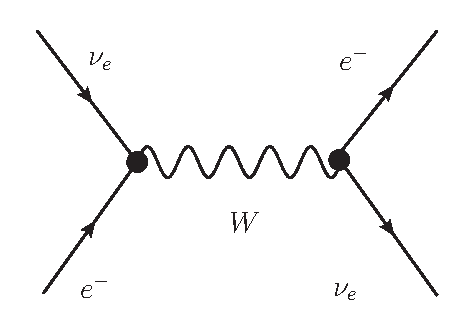
\includegraphics[width=4.5cm]{charged-1.eps}
	\end{minipage}
	\begin{minipage}[t]{0.3\textwidth}{(b)}
		\centering
		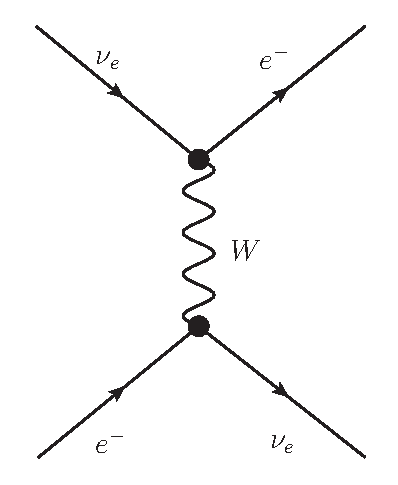
\includegraphics[height=4cm]{charged.eps}
	\end{minipage}
	%	\begin{minipage}[t]{0.4\textwidth}{(c)}
	%	\centering
	%	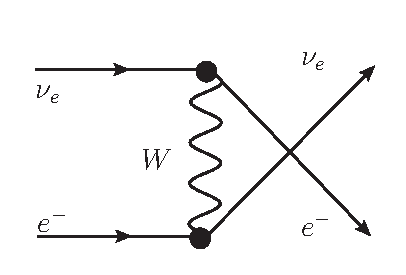
\includegraphics[width=4.5cm]{charged-u.eps}
	%\end{minipage}
	\begin{minipage}[t]{0.4\textwidth}{(c)}
		\centering
		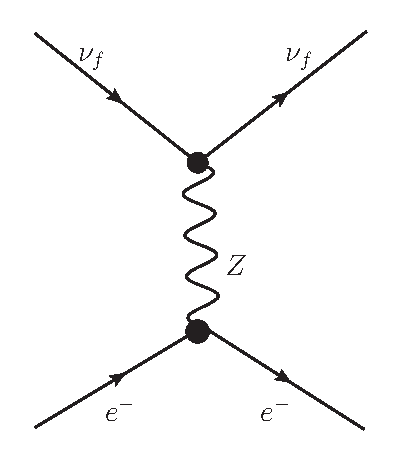
\includegraphics[height=4cm]{neutral.eps}
	\end{minipage}
	\caption[Feynman diagrams for different channels of the elastic scattering interaction.]{Feynman diagrams for different channels of the elastic scattering interaction at tree level. (a) and (b): charged current for s and t channels, respectively; (c): neutral current.}
	\label{feynman-es}
\end{figure}

charged-current, the charged vector bosons $W^\pm$ 


neutral-current, the neutral vector boson $Z^0$


neutrino-electron elastic scattering ($\nu e^-$ ES)
\begin{equation}
\nu_x + e^{-}\to\nu_x+e^-,
\end{equation}
is sensitive to all neutrino flavors, but $\nu_e$ has channels of (a) and (b)

the cross-section is 6.5 times larger than the $\nu_{\mu,\tau}$.


In a particle detector, the electron is usually from the atom of detection medium. 

\begin{equation}
\frac{d\sigma}{dT_e}=\frac{2G_F^2m_e}{\pi}[g_L^2+g_R^2\left(1-\frac{T_e}{E_\nu}\right)^2-g_Lg_R\frac{m_eT_e}{E_\nu^2}],
\end{equation}
where the coupling parameters $g_L=(\sin^2\theta_W\pm\frac{1}{2})$, $g_R=\sin^2\theta_W$, $\sin^2\theta_W=0.23$.

In the laboratory frame, the kinetic energy of a recoil electron from the $\nu e^-$ ES process is\cite{giunti2007fundamentals}:
\begin{equation}
T_e = \frac{2m_eE_\nu^2\cos\theta}{(m_e+E_\nu)^2-E_\nu^2\cos^2\theta},
\end{equation}
where the scattering angle $\theta$ is between the incoming neutrino direction and the outgoing electron direction.

$T_{max}=\frac{2E^2_\nu}{2E_\nu+m_e c^2}$
the cross-section is $\sigma(\nu_e+e^-\to \nu_e+e^-)=9.52\times 10^{-44}(E_\nu/10~MeV)~cm^2$
the expected solar neutrino rate is 
$R=A\int_{T_{thresh}}^{T_{max}}\frac{d\sigma}{dE}\frac{dN}{dE_\nu}dE_\nu$.

The direction of the scattered electron is correlated with the direction of the incident neutrino. 
$\nu-e^-$ elastic scattering: 
\begin{equation}\label{eq:costhetaSun}
\cos\theta_{sun}=\sqrt{\frac{T_e(m_e+E_\nu)^2}{2m_eE_\nu^2+T_eE_\nu^2}},
\end{equation}

conservation of momentum

For the solar neutrinos, the momentum of the recoil electrons are strongly pointing away from the Sun.
\begin{figure}[htbp]
	\centering	
	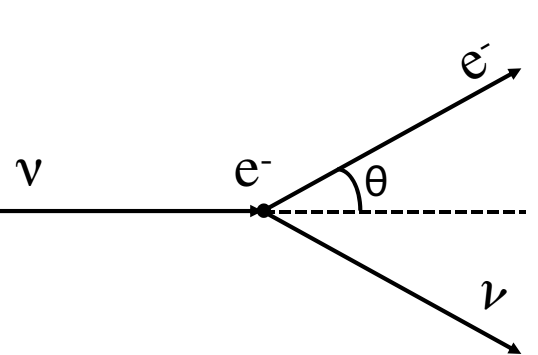
\includegraphics[width=6cm]{ElasticScatteringCartoon.png}
	\caption{A diagram of the $\nu e^-$ elastic scattering in the lab frame.}
	\label{fig:ESdiagram}
\end{figure}

%In the next two sections, I will show the two properties which are under the spotlight: neutrinos can change their flavors and they have masses.

\section{Neutrino Flavor Transformation}
Neutrino flavor transformation is a quantum mechanical interference phenomenon\cite{akhmedov2019quantum}. It was first discovered in 1998, based on the analysis of atmospheric neutrino fluxes measured by the Super-Kamiokande (Super-K) experiment to solve the ``atmospheric neutrino anomaly'' mentioned in the last section\cite{sect:fukuda1998evidence}. It is the first direct evidence showing that neutrinos have finite masses and the SM is incomplete.

\subsection{Vacuum Oscillation}\label{sectVacuumOsci}
For neutrino flavor oscillation experiments, neutrinos are detected in certain flavor eigenstates via weak interaction. A neutrino flavor state vector can be taken as a linear superposition of the mass eigenstates. For three-flavor neutrino mixing, we have\cite{pdg2020}:
\begin{equation}\label{eq:mixingmatrix}
|\nu_f\rangle = \sum_{i=1}^3U^*_{fi}|\nu_i\rangle, 
\end{equation}
where $f=e,\mu,\tau$ and $k=1,2,3$. The unitary PMNS matrix, $U_{PMNS}$, can be parameterized as\footnote{Here we ignore the Majorana CP violation phases, which are cancelled out when tackling with the flavor transformation probability. We will come to this part in Sect.~\ref{section:Majorana}}: 
\begin{equation}\label{eq:uPMNS}
U_{PMNS} =
\begin{pmatrix}
1 &0 &0\\
0 &c_{23} &s_{23}\\
0 &-s_{23} &c_{23}\\ 
\end{pmatrix}
\begin{pmatrix}
c_{13} &0 &e^{-i\delta_{CP}}s_{13}\\
0 &1 &0\\
e^{-i\delta_{CP}}s_{13} &0 &c_{13}\\ 
\end{pmatrix}
\begin{pmatrix}
c_{12} &s_{12} &0\\
-s_{12} &c_{12} &0\\
0 &0 &1\\ 
\end{pmatrix},
\end{equation}
where $c_{ij}\equiv \cos\theta_{ij}$ and $s_{ij}\equiv \sin\theta_{ij}~(i,j = 1,2,3)$ are shorthands.
In the PMNS matrix, there are four parameters: the three mixing angles $\theta_{12}$, $\theta_{13}$, $\theta_{23}$ and the charge-parity (CP) violation parameter of lepton sector, $\delta_{CP}$. The unknown value of $\delta_{CP}$ is related to leptogenesis, the hypothetical physical process that produced an asymmetry between leptons and anti-leptons in the very early universe\cite{wiki_cp}. 

Now discuss the vacuum flavor oscillation: in the lab frame, assume a neutrino is generated at time $t_0=0$ from a source with a certain flavor state $|\nu_\alpha\rangle$. It then propagates in vacuum with a speed close to the speed of light (ultra-relativistic) for a distance $L$ and is finally detected at time $t$ in a detector. The flavor eigenstate evolves in space-time is $|\nu_\alpha \rangle = \sum_i U^*_{\alpha i}|\nu_i,p_i\rangle$, where $p_i$ is the 4-momentum of $\nu_i$. The momentum is assumed to be along the direction from the source to the detector and only in one dimension. Via the Schr\"{o}dinger equation, the amplitude for the flavor eigenstate $|\nu_\beta>$ in the detector at $(L,t)$ is (use the natural units: $\hbar=c=1$) \cite{aitchison2012gauge}:
\begin{equation}
\mathcal{A}(\nu_\alpha\to\nu_\beta;L,E)=\sum_{i}U^*_{\alpha i}e^{-iE_i t+ip_iL}\langle\nu_\beta|\nu_i,p_i\rangle=\sum_{i}U^*_{\alpha i}U_{\beta i}e^{-iE_it+ip_iL},
\end{equation}

Then the probability of $\nu_\alpha$ at time $t_0=0$ transforms into a $\nu_\beta$ at time $t$ is:
\begin{equation}\label{oscillationEq1}
 \begin{split}
&P(\nu_\alpha\to\nu_\beta;L,E)=|\langle\mathcal{A}(\nu_\alpha\to\nu_\beta;L,E)|\mathcal{A}(\nu_\alpha\to\nu_\beta;L,E)\rangle|^2=\\
&(U^*_{\alpha 1}U_{\beta 1}e^{-iE_1t+ip_1L}+U^*_{\alpha 2}U_{\beta 2}e^{-iE_2t+ip_2L}+...)(U_{\alpha 1}U^*_{\beta 1}e^{+iE_1t-ip_1L}+U_{\alpha 2}U^*_{\beta 2}e^{+iE_2t-ip_2L}+...)=\\
&\sum_i |U_{\alpha i}|^2|U_{\beta i}|^2 + \sum_{i>j}(U^*_{\alpha i}U_{\beta i}U_{\alpha j}U^*_{\beta j})\exp\{-i(E_i-E_j)t+i(p_i-p_j)L\}+(i\leftrightarrow j),
\end{split}
\end{equation}
where $(i\leftrightarrow j)$ stands for the second term exchanging the $i,j$ indices.

For the second term in Eqn.~\ref{oscillationEq1}, in the ultra-relativistic case, $p_i\simeq p_j\equiv p\simeq E\gg m$, where $E$ is the average energy. Then $E_i=\sqrt{p^2_i+m^2_i}\simeq p+\frac{m_i^2}{2E}$ and thus $E_i-E_j\simeq \frac{m^2_i-m^2_j}{2E}\equiv \frac{\Delta m^2_{ij}}{2E}$\cite{pdg2020,aitchison2012gauge}. Here $\Delta m^2_{ij}$ is a set of parameters called mass square difference, popping out in the flavor transition probability. Along with $L\simeq ct=t~(c\equiv 1)$, we have $\exp\{-i(E_i-E_j)t+i(p_i-p_j)L\}\simeq \exp\{-i\frac{\Delta m^2_{ij}}{2E}\}$. In addition, $U^*_{\alpha i}U_{\beta i}U_{\alpha j}U^*_{\beta j}=|U^*_{\alpha i}U_{\beta i}U_{\alpha j}U^*_{\beta j}|\exp\{i\phi_{\alpha\beta;ij}\}$, where $\phi_{\alpha\beta;ij}=\mathrm{Arg}(U^*_{\alpha i}U_{\beta i}U_{\alpha j}U^*_{\beta j})$ and $\phi_{\alpha\beta;ij}=-\phi_{\alpha\beta;ji}$. Then combine the second term and the $(i\leftrightarrow j)$ term, \ref{oscillationEq1} can be written as\cite{aitchison2012gauge}:
\begin{equation}\label{oscillationEq2}
P_{\nu_\alpha\to\nu_\beta}(L,E)=
\sum_i |U_{\alpha i}|^2|U_{\beta i}|^2 + 2\sum_{i>j}|U^*_{\alpha i}U_{\beta i}U_{\alpha j}U^*_{\beta j}|\cos(\frac{\Delta m^2_{ij}}{2E}L-\phi_{\alpha\beta;ij}).
\end{equation}

Further expand the second term in Eqn.~\ref{oscillationEq2}:
\begin{equation}
 \begin{split}
&|U^*_{\alpha i}U_{\beta i}U_{\alpha j}U^*_{\beta j}|\{\cos(\phi_{\alpha\beta;ij})\cos(\frac{\Delta m^2_{ij}}{2E}L)+\sin(\phi_{\alpha\beta;ij})\sin(\frac{\Delta m^2_{ij}}{2E}L)\}=\\
&\Re(U^*_{\alpha i}U_{\beta i}U_{\alpha j}U^*_{\beta j})(1-2\sin^2\frac{\Delta m^2_{ij}L}{4E})+\Im(U^*_{\alpha i}U_{\beta i}U_{\alpha j}U^*_{\beta j})\sin\frac{\Delta m^2_{ij}L}{2E},
 \end{split}
\end{equation}

since the matrix $U$ is unitary and when $t=0$, 
\begin{equation}
P_{\nu_\alpha\to\nu_\beta}=\delta_{\alpha\beta}=\sum_i |U_{\alpha i}|^2|U_{\beta i}|^2+2\sum_{i>j}\Re(U^*_{\alpha i}U_{\beta i}U_{\alpha j}U^*_{\beta j}),
\end{equation} 

finally it comes out the commonly used vacuum oscillation equation\cite{pdg2020,aitchison2012gauge}:
\begin{equation}\label{common_oscillation}
P_{\nu_\alpha\to\nu_\beta}(L,E)=\delta_{\alpha\beta}-4\sum_{i>j} \Re[U_{\beta i}U^*_{\alpha i}U_{\alpha j}U^*_{\beta j}]\sin^2\frac{\Delta m^2_{ij}L}{4E}+2\sum_{i>j} \Im(U_{\beta i}U^*_{\alpha i}U_{\alpha j}U^*_{\beta j})\sin\frac{\Delta m^2_{ij}L}{2E}.
\end{equation}

Choose a set of units commonly used by experiments and with dimensional transformation, we have\cite{pdg2020}:
\begin{equation}
X_{ij}\equiv \frac{\Delta m^2_{ij}L}{4E}=\frac{1.267\Delta m_{ij}^2[eV^2]L[m]}{E_\nu[MeV]}.
\end{equation}

Maximum oscillation occurs when $X_{ij}\sim \pi$, which gives an effective length $L^{osc}(\Delta m_{ij},E_\nu)=4\pi E/|\Delta m_{ij}^2|$.

Currently, the four parameters in the PMNS matrix, as well as the parameters of the $\Delta m_{ij}$, have been measured by neutrino oscillation experiments. These experiments can be classified by the neutrino sources they use. They are the solar, the reactor, the atmospheric, the accelerator, and the astronomical and cosmological neutrino experiments. Table~\ref{nu_exp} lists the energy scale of the neutrino source as well as the example experiments.

\begin{table}[ht]
	\caption{\label{nu_exp} Oscillation neutrino experiments.}	
	{\centering
		\begin{tabular*}{135mm}{c@{\extracolsep{\fill}}cccc}
			\toprule 
			type & source & $E_\nu$ & example\\
			\midrule
			solar& the Sun & MeV scale & SNO \\
			reactor& reactor & MeV scale & DayaBay \\
			atmospheric& cosmic-ray& GeV scale & SuperK\\
			accelerator&  $\nu$ beam from accelerator & GeV scale & T2K\\	
			astronomical& astronomical objects & GeV-EeV scale & IceCube\\	
			\bottomrule	
		\end{tabular*}
	}
\end{table}

For the $\Delta m^2_{21}$ and $\theta_{12}$, the combined analysis of the measurements from the reactor experiment KamLAND and SNO gave $\Delta m^2_{21} = 7.59^{+0.21}_{-0.21}\times 10^{-5}eV^2$ and $\tan^2{\theta}_{21}=0.47^{+0.06}_{-0.05}$\cite{abe2008precision}.

The accelerator neutrino experiments as well as the atmospheric neutrino experiments have measured $\Delta m^2_{32}$ and $\theta_{23}$. The most recent results from SuperK show that in NH, $\sin^2\theta_{23}=0.588^{+0.031}_{-0.064}$ and $\Delta m^2_{32} = 2.5^{+0.13}_{-0.20}\times 10^{-3} eV^2$\cite{abe2018atmospheric}. 

In 2012, the reactor neutrino experiment Daya Bay reported the discovery of non-zero $\theta_{13}$ with a significance of 5.2$\sigma$. In 2016, Daya Bay reported that $\sin^2 2\theta_{13} = 0.0841\pm0.0027(stat.)\pm0.0019(syst.)$. This high-precision result makes $\sin^2 2\theta_{13}$ the best measured mixing angle\cite{an2017measurement,qian2019physics}.

In addition, there are two squared-mass differences, $\Delta m^2_{21}=m_2^2-m_1^2$ and $\Delta m^2_{32}=|m_3^2-m_2^2|$. The sign of $\Delta m^2_{32}$ is unknown and it indicates a mass hierarchy problem of whether neutrino mass is normal hierarchy (NH, $m_3>m_2>m_1$) or inverted hierarchy (IH, $m_3<m_1<m_2$)\cite{pdg2020}. 

$L/L^{osc}(\Delta m_{31},E_\nu)\sim 1$ and $L/L^{osc}(\Delta m_{21},E_\nu)\ll 1$
\begin{equation}
P_{\nu_\alpha \to \nu_\beta}(L,E)\simeq \delta_{\alpha\beta}-4|U_{\alpha3}|^3(\delta_{\alpha\beta}-|U_{\beta 3}|^2)\sin^2\frac{\Delta m^2_{31}L}{4E}=P_{\bar{\nu}_\alpha \to \bar{\nu}_\beta}(L,E)
\end{equation}

In the case of antineutrino flavor oscillation, we have: $|\bar{\nu}_\alpha>=\sum_i U_{\alpha i}|\bar{\nu}_i,p_i>$, via the same calculation, a similar oscillation probability equation can be found but with the last term in \ref{common_oscillation} being negative\cite{aitchison2012gauge}:
\begin{equation}\label{antiNu_eq1}
P_{\bar{\nu}_\alpha\to\bar{\nu}_\beta}(L,E)=\delta_{\alpha\beta}-4\sum_{i>j} \Re[U_{\beta i}U^*_{\alpha i}U_{\alpha j}U^*_{\beta j}]\sin^2\frac{\Delta m^2_{ij}L}{4E}-2\sum_{i>j} \Im(U_{\beta i}U^*_{\alpha i}U_{\alpha j}U^*_{\beta j})\sin\frac{\Delta m^2_{ij}L}{2E}.
\end{equation}

This provides a measure of CP violation\cite{aitchison2012gauge}:
\begin{equation}\label{cpV_eq1}
%\begin{split}
\mathcal{A}_{CP}=P_{\nu_\alpha\to\nu_\beta}(L,E)-P_{\bar{\nu}_\alpha\to\bar{\nu}_\beta}(L,E)=
4\sum_{i>j} \Im(U_{\beta i}U^*_{\alpha i}U_{\alpha j}U^*_{\beta j})\sin\frac{\Delta m^2_{ij}L}{2E}.
%\end{split}
\end{equation}

\cite{antonio2018state}

$\delta_{CP}$ is examined by the experiments which measure the difference between neutrino and antineutrino oscillation probabilities $P(\bar{\nu}_\alpha\to\bar{\nu}_\beta)$ and $P(\nu_\alpha\to\nu_\beta)$\cite{xing2011neutrinos}. In 2017, the Tokai-to-Kamioka (T2K) experiment in Japan rejected the hypothesis that neutrinos and antineutrinos oscillate with the same probability at 95\% confidence (2$\sigma$) level. This indicates a hint of CP symmetry broken by neutrinos\cite{abe2017measurement}. In 2019, T2K  claimed confidence intervals for $\delta_{CP}$ with three standard deviations ($3\sigma$): [-3.41,-0.03] for NH and [-2.54,-0.32] for IH. This result indicates that the CP violation exists in leptons\cite{abe2019constraint}.

\subsection{Matter Effect}
The matter effect is caused by neutrinos interacting with ambient electrons and nucleons in the matter such as the Sun or the Earth. $\nu_e$ interacts with electrons via both charged weak current (exchanging $W$ boson) and neutral weak current ($Z$ boson) while $\nu_\mu$ and $\nu_\tau$ interact only by the neutral current. The $\nu_e$ energy has an addition term, $V_{CC} =\sqrt2G_Fn_e$, where $n_e$ is the number density of the electrons in matter and $G_F$ is the Fermi coupling constant for the weak interaction. This affects the oscillation probabilities for neutrinos propagating in matter compared to vacuum, which is called the Mikheyev-Smirnov-Wolfenstein (MSW) mechanism\cite{smirnov2016solar,smirnov2005msw}.

In vacuum two-flavor mixing, the Schr\"{o}dinger equation can be written (in natural units)\cite{xing2011neutrinos}:
\begin{equation}\label{eq:2flavor_simple}
	i\frac{d}{dt}\begin{pmatrix}
		\nu_e\\
		\nu_\mu\\
	\end{pmatrix}
	=
	H^f_0
	\begin{pmatrix}
		\nu_e\\
		\nu_\mu\\
	\end{pmatrix},
\end{equation}

\begin{equation} \label{eq:H0f}
\begin{aligned}
 H^f_0 = \frac{1}{2E}\begin{pmatrix}m^2_1\cos^2\theta+m^2_2\sin^2\theta & (m^2_2-m^2_1)\sin\theta\cos\theta \\ (m^2_2-m^2_1)\sin\theta\cos\theta & m^2_1\sin2\theta+m^2_2\cos^2\theta\end{pmatrix} =
\\
\frac{\Delta m_{21}^2}{4E}\begin{pmatrix}
	-\cos 2\theta & \sin 2\theta\\
	\sin 2\theta & \cos 2\theta\\
\end{pmatrix}+\frac{(m_1^2+m_2^2)}{4E}\begin{pmatrix}
	1 & 0\\
	0 &1\\
\end{pmatrix},
\end{aligned}
\end{equation}
and $\Delta m^2_{21}=(m^2_2 - m^2_1)$.

To simplify the calculation, we can drop the second unitary term of $H^f_0$ that is irrelevant to the neutrino flavor transformation. Including the matter effect, we obtain:
\begin{equation}\label{eq:Hm}
	H_m = \begin{pmatrix}
		-\frac{\Delta m_{21}^2}{4E}\cos 2\theta+\sqrt 2G_Fn_e & \frac{\Delta m_{21}^2}{4E}\sin 2\theta\\
		\frac{\Delta m_{21}^2}{4E}\sin 2\theta &\frac{\Delta m_{21}^2}{4E}\cos 2\theta\\
	\end{pmatrix}
\end{equation}

We define a mixing angle in matter, $\theta_m$ as:
\begin{equation}\label{eq:thetaM}
	\tan 2\theta_m = \frac{\Delta m^2\sin2\theta}{\Delta m^2\cos2\theta-2\sqrt 2E G_Fn_e},
\end{equation}
and define an effective squared-mass difference in matter $\Delta m^2_m$ as:
\begin{equation}
	\Delta m^2_m = \sqrt{(\Delta m^2\cos2\theta - 2\sqrt 2EG_Fn_e)^2+(\Delta m^2\sin2\theta)^2}.
\end{equation}

In analogy with mixing in vacuum, we can write the mixing equation relating the energy eigenstates in matter ($\nu_{1m},\nu_{2m}$) to the flavor eigenstates with a diagonalized Hamiltonian:
\begin{equation}\label{eq:matter_mixing}
	\begin{pmatrix}
		\nu_e\\
		\nu_\mu\\
	\end{pmatrix}
	= \begin{pmatrix}
		\cos\theta_m & \sin\theta_m\\
		-\sin\theta_m & \cos\theta_m \\
	\end{pmatrix}
	\begin{pmatrix}
		\nu_{1m}\\
		\nu_{2m}\\
	\end{pmatrix}.
\end{equation}

The probability of flavor transformation in matter is:
\begin{equation}
	P_{\nu_e\to\nu_{\mu}}=\sin^2(2\theta_m)\sin^2\Big(\frac{\Delta m_m^2L}{4E}\Big).
\end{equation}

The denominator in equation (\ref{eq:thetaM}) implies a resonance condition:
\begin{equation}\label{eq:reson_condition}
	V(n_e)=\sqrt 2G_Fn_e=\frac{\Delta m^2\cos2\theta}{2E}.
\end{equation}

From this condition, for a given $E$, there is a resonance density $n^{reson}_e$ while for a given $n_e$, there is a resonance energy $E^{reson}$. When the resonance condition is satisfied, $\theta_m = \frac{\pi}{4}$ and two flavor neutrinos are maximally mixed, even if the vacuum mixing angle $\theta$ is small. This is called matter enhanced neutrino oscillation\cite{smirnov2016solar,fukugita2013physics}, which was observed from measuring the solar neutrinos. I will discuss it in the next two sections.

%The oscillation probability in matter can be written in a concise and exact form as \cite{kimura2002exact}:
%\[
%P(\nu_e\to\nu_\mu) = A\cos\delta+B\sin\delta+C
%\]
%
%will also provide the information for the CP- and T-violation
%by investigating the quantities of:
%\[
%A_{CP} = \frac{P(\nu_\alpha\to\nu_\beta)-P(\bar{\nu}_\alpha\to\bar{\nu}_\beta)}{P(\nu_\alpha\to\nu_\beta)+P(\bar{\nu}_\alpha\to\bar{\nu}_\beta)}
%\]
%
%\[
%A_T = \frac{P(\nu_\alpha\to\nu_\beta)-P(\bar{\nu}_\beta\to\bar{\nu}_\alpha)}{P(\nu_\alpha\to\nu_\beta)+P(\bar{\nu}_\beta\to\bar{\nu}_\alpha)}
%\]

Table~\ref{table:nuOscillation} summarizes the types of experiments for neutrino flavor transformation and the relating parameters\cite{giunti2007fundamentals,nagashima2014beyond}.
\vspace{1mm}
\begin{table}[ht]
	\centering
	\caption{}
	\label{table:nuOscillation}
	\begin{tabular}{ccccc}
		\toprule
		Source & Energy ($\mathcal{O}$(MeV)) & Distance ($\mathcal{O}$(m)) &  $\Delta m^2$ ($\mathcal{O}$(eV$^2$)) \\
		\hline 
	Accelerator & $10^3-10^5$ & $10-10^7$ & $10^{-3}-100$\\	
		\hline 
    Reactor	& 1 & $10^2-10^3$ & $10^{-5}-0.1$\\			
	 \hline 
	Cosmic ray	& $10^3$ & $10^7$ & $10^{-4}$\\		
	\hline
	Sun & 1 & $10^{11}$ & $10^{-11}$\\	
	 \hline
	Supernova & 1-10 & $10^2-10^3$ & $10^{-20}$\\	
 \bottomrule
	\end{tabular}
\end{table}
\vspace{1mm}

\subsection{Solar Neutrinos}
Since the Sun is an object provides ambient electrons and nucleons, neutrinos coming from the Sun are traditionally used to investigate the matter effects.

In the 1930s, Hans Bethe et al. explained the origin of the Sun's energy as a series of nuclear reactions\cite{bethe1939energy}.

Based on the available physics and experimental data, the Standard Solar Model (SSM) is a modern accepted theory for the evolution of the Sun. The energy in the Sun is mainly produced by two sets of reactions: the proton-proton (pp) chain, which contributes to $\sim 98.6\%$ of the energy release and the Carbon-Nitrogen-Oxygen (CNO) cycle, which contributes $\sim 1.4\%$. Fig.~\ref{ppChain} and Fig.~\ref{CNOcycle} show all the reactions in the two sets respectively. Via these two main sets of nuclear reactions, hydrogen is eventually fused into helium, and the net nuclear transformation is $4p+2e^-\to^{4}$He $+2\nu_e+Q$, where the released energy $Q=26.73$ MeV is mostly in the form of the kinetic energy of the photons, with a small fraction carried by neutrinos\cite{valle2015neutrinos,antonio2018state}. The average energy of solar $\nu_e$ is calculated by summing over the $E_{\nu_e}$ from the $i^{th}$ reaction chain with a flux of $\Phi_{\nu_e}^i$ and divided by $\Phi^{tot}_{\nu_e}$

%reaction chains. For 
%
%as\cite{antonio2018state}:
\begin{equation}
\langle E_{\nu_e}\rangle = \sum_i E_i \frac{\Phi^i_{\nu_e}}{\Phi^{tot}_{\nu_e}}\approx 0.265~MeV,
\end{equation}

(the average neutrino energy $\langle E_{2\nu_e} \rangle\sim 0.59$ MeV). 

Besides, about 2 MeV of $Q$ is from annihilation of positrons with electrons in the solar plasma\cite{valle2015neutrinos,antonio2018state}. For every released energy, there are about 2 $\nu_e$ generated. The solar $\nu_e$ flux at the Earth surface can be estimated via the measured solar radiation energy on the Earth surface:
\begin{equation}
\Phi_{\nu_e} \simeq \frac{2\mathcal{L}_{\odot}}{4\pi D_\odot^2}\frac{1}{Q-2\langle E_{\nu_e} \rangle}= 6.35\times 10^{10}~\nu_e/cm^2/s,
\end{equation}

where the solar constants $G_{sc}=\mathcal{L}_\odot/(4\pi D^2_\odot)\simeq 0.136$ W/cm$^2$ \cite{suekane2015neutrino}. 

The electron neutrinos produced in the solar nuclear reactions are named solar neutrinos and they can be detected on the Earth. Due to the branching ratios and unterminated chains in the pp chain and CNO cycle, the solar neutrinos come from different reactions, as shown in Table~\ref{solarnu}. The specific solar neutrinos detected on the Earth are named after the specific fusion process\cite{haxton2013solar}. They have different fluxes and energies, as shown in Fig.~\ref{bp05plot}\cite{bahcall2005new}.

\begin{figure}[htbp]
	\centering	
	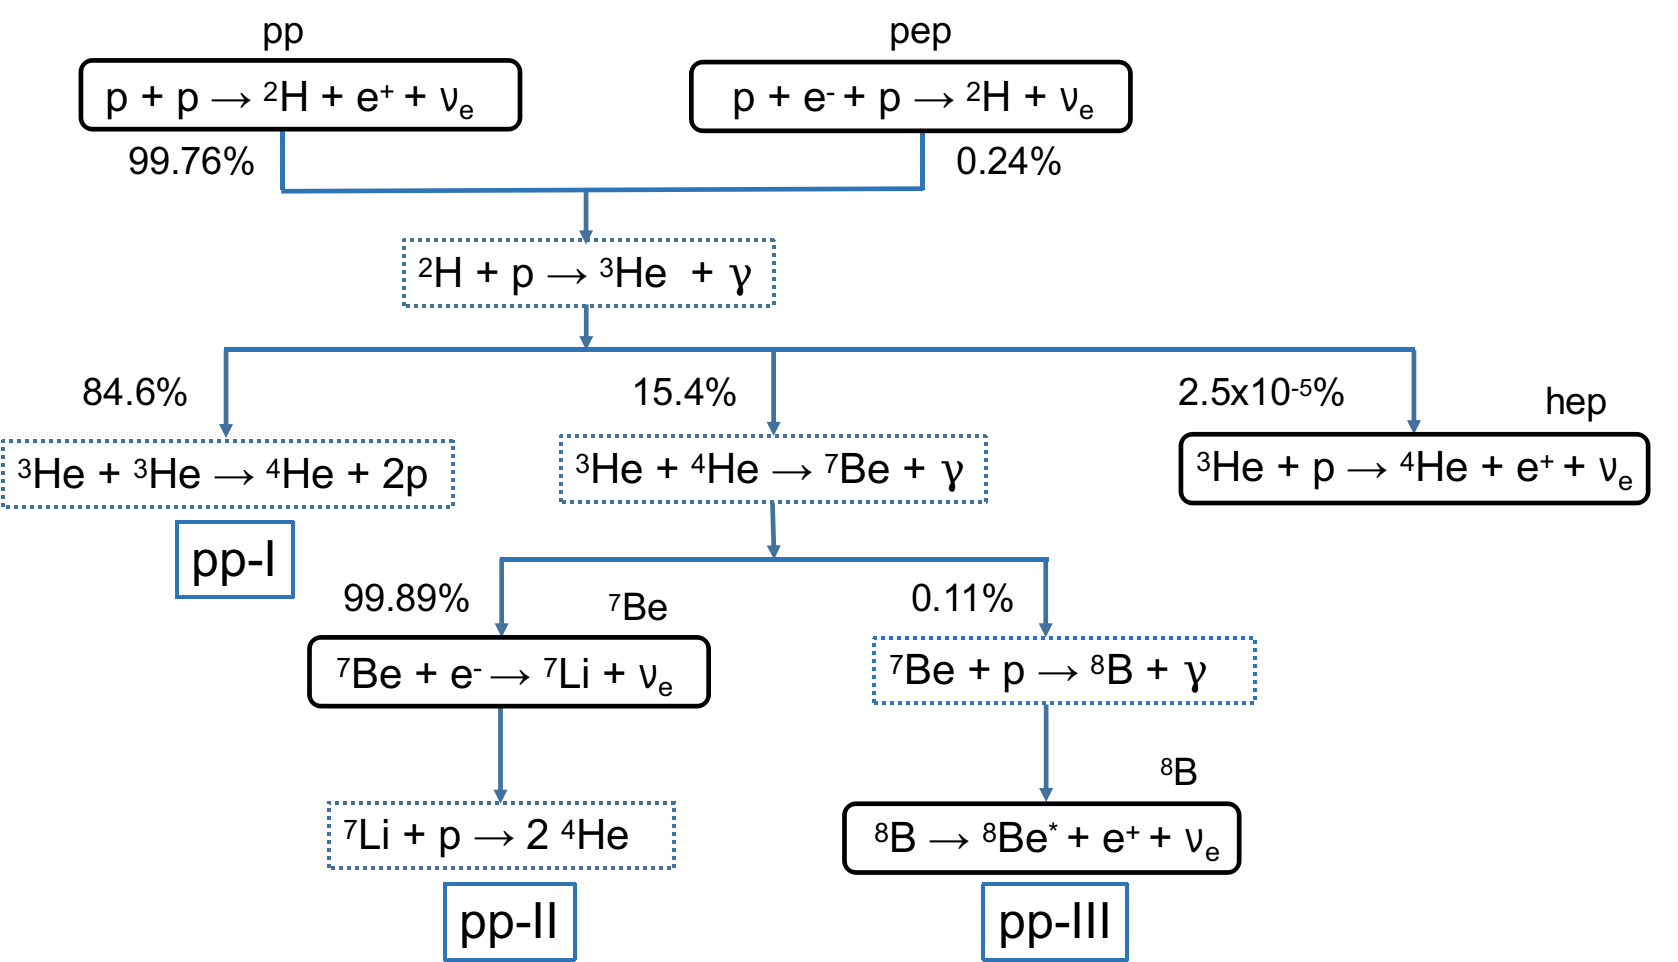
\includegraphics[width=14cm]{ppChain.png}
	\caption[All reactions in the three PP chains.]{All reactions in the three PP chains: PP-I, PP-II, PP-III. The reactions producing neutrinos are labeled in the solid frames. Modified from \cite{oberauer2020solar}.}
	\label{ppChain}
\end{figure}

\begin{figure}[htbp]
	\centering	
	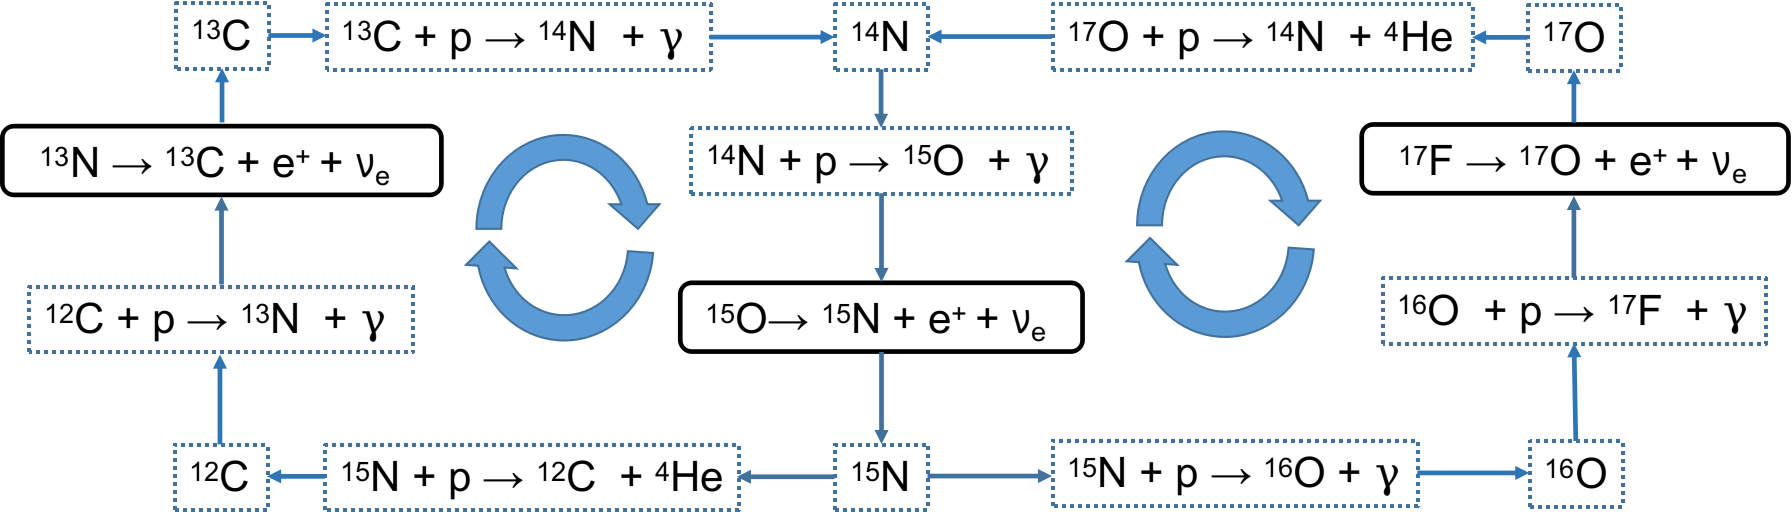
\includegraphics[width=14cm]{CNOcycle.png}
	\caption[All reactions in the CNO bicycle.]{All reactions in the CNO bicycle. The reactions producing neutrinos are labeled in the solid frames. Modified from \cite{oberauer2020solar}.}
	\label{CNOcycle}
\end{figure}

\begin{table}[htp]
	\caption[]{\label{solarnu} Solar neutrinos from reactions in pp chain (a) and CNO cycle (b).}	
	\subfigure[pp chain]{
		\begin{tabular*}{62mm}{cc}
			\toprule 
			solar $\nu_e$  & reaction  \\
			\midrule
			pp & $p+p\to ^2$H $+e^++\nu_e$ \\
			pep & $p+e^-+p\to^2$H $+~\nu_e$ \\
			hep &  $^3$He $+~p\to^4$He $+~e^++\nu_e$ \\ 
			$^7$Be &  $^7$Be $+~e^-\to^7$Li $+~\nu_e$\\
			$^8$B & $^8$B$\to^8$Be$^*+e^++\nu_e$\\
			\bottomrule	
		\end{tabular*}
	}
	\subfigure[CNO cycle]{
		\begin{tabular*}{60mm}{cc}
			\toprule 
			solar $\nu_e$   & reaction \\
			\midrule
			CNO &$^{13}$N$\to^{13}$C$+e^++\nu_e$\\	
			& $^{15}$O$\to^{15}$N$+e^++\nu_e$ \\
			& $^{17}$F$\to^{17}$O$+e^++\nu_e$ \\
			\bottomrule	
		\end{tabular*}
	}
\end{table}

\begin{figure}[htbp]
	\centering	
	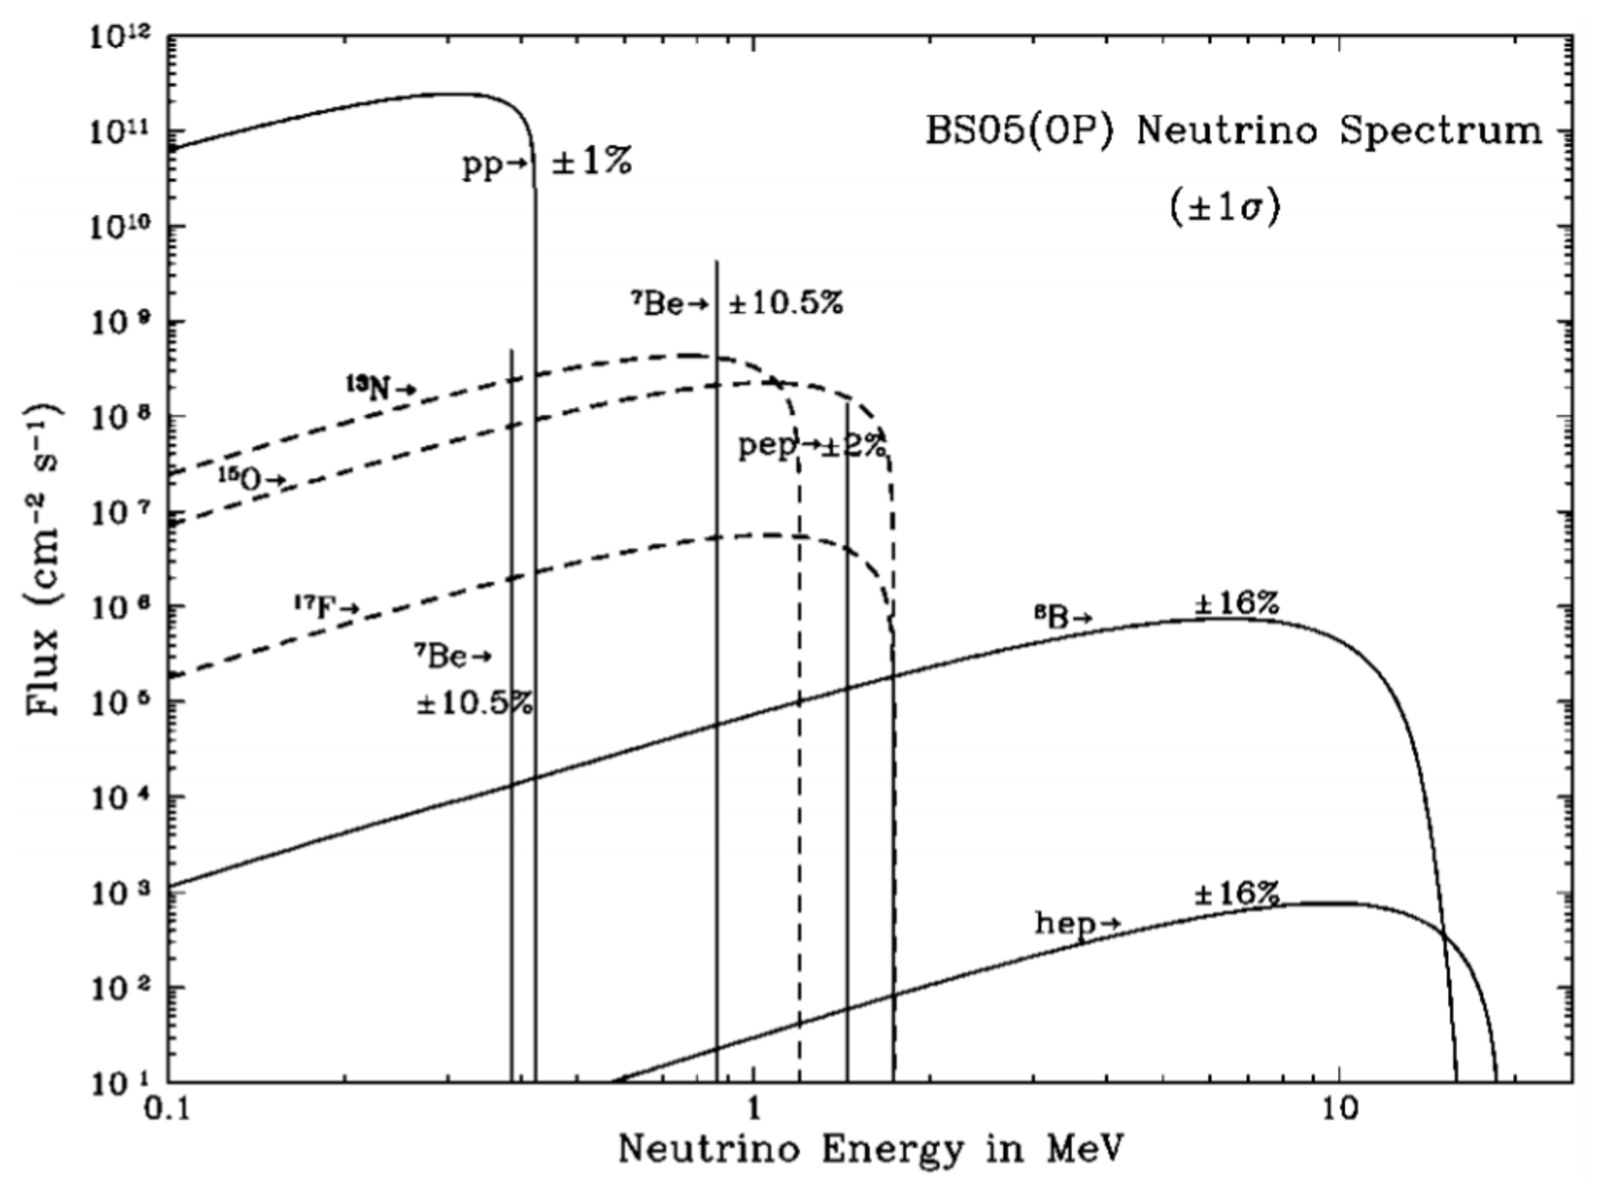
\includegraphics[width=10cm]{BP05.pdf}
	\caption[Solar neutrino energy spectrum based on BS05(OP).]{Solar neutrino energy spectrum ($E_\nu$ vs. flux) based on the solar model BS05(OP). Figure is from Ref.~\cite{bahcall2005new}.}
	\label{bp05plot}
\end{figure}
solar neutrinos are also major backgrounds to the $0\nu\beta\beta$ search



\subsection{Status of the Neutrino Flavor Transformation Experiments}
In 1964, John Bahcall and Raymond Davis proposed the first experiment to detect solar neutrinos\cite{bahcall1964solar,davis1964solar}. Raymond Davis designed an experiment that used a 380 m$^3$ tank filled with Perchloroethylene (C$_2$Cl$_4$), a dry-cleaning fluid rich in chlorine. Solar neutrinos were expected to change $^{37}$C1 to $^{37}$Ar via the endothermic reaction $\nu_e+^{37}$Cl$\to^{37}$Ar$+e^-$ and the produced $^{37}$Ar were extracted and counted. The neutrino energy threshold ($E_{thresh}$) of the experiment was 0.814 MeV, which allowed a measurement mostly of the $^8$B neutrino flux but also including some lower energy neutrinos\cite{davis1964solar}. Their first results, announced in 1968, showed that only about one-third of the predicted radioactive argon atoms were measured. This raised the problem of missing solar neutrinos.

%\subsection{Atmospheric Neutrino}
%Cosmic rays from outer space continuously interact with nuclei in the atmosphere and produce secondary particles. Atmospheric neutrinos come from decay products of the hadrons in the secondaries. The dominant processes of atmospheric $\nu_e$ and $\nu_\mu$ production is $\pi^+\to\mu^+ + \nu_\mu$ followed by $\mu^+ \to e^+ + \bar{\nu}_\mu + \nu_e$. In the 1980s, the Kamiokande experiment in Japan measured atmospheric neutrinos by utilizing a 3-kiloton water-Cherenkov detector. The incoming neutrinos, $\nu_e$ ($\nu_\mu$) interacted with the water via charged current interactions, and electrons (muons) were produced. The electrically charged leptons traversed the water at a speed higher than the speed of light in water and thus emit Cherenkov light, which was recorded by the detector as ring patterns (called Cherenkov rings). The produced electrons caused electromagnetic showers during their propagation in the water while the produced muons propagated almost in straight lines without producing electromagnetic showers. Then the $\nu_\mu$ (the $\mu$-like events) were separated from the $\nu_e$ (the $e$-like events) by the fact that the $\mu$-like events created sharper Cherenkov rings than the $e$-like events. Kamiokande measured the ratio of fluxes $\Phi(\nu_\mu+\bar{\nu}_\mu)/\Phi(\nu_e+\bar{\nu}_e)$. The fluxes of atmospheric neutrinos are well understood and the ratio $\nu_\mu/\nu_e$ is expected to be $\sim$2 at low energies $\leq$1~GeV. In 1988, they found a deficit of measured $\mu$-like events compared to the prediction. This was later confirmed by IMB in 1992\cite{becker1992electron} and Soudan-2 in 1997\cite{allison1997measurement} and called ``atmospheric neutrino anomaly''\cite{kajita2012atmospheric}.
\subsection{SNO}

Since neutrinos' extremely low interaction cross-sections, neutrinos produced in the Sun can reach the detectors on the Earth without being interrupted. This enables the solar neutrino to be a probe to stellar physics.

A combined analysis of three phases of SNO data shows that the measured total flux is $5.25\pm0.16^{+0.11}_{-0.13}~cm^{-2}s^{-1}$.

\subsection{Super-Kamiokande}
SuperK

15 $\nu$ events/day.

For the $^8$B solar neutrino flux, SuperK reported a measurement of $(2.345\pm0.014\pm0.036)\times 10^6~cm^{-2}s^{-1}$.

\subsection{Borexino}

Borexino reported the first observation of CNO neutrino in 2020

interaction rate is $7.2^{+3.0}_{-1.7}$ counts per day per 100 tonnes of target at 68\% C.L. This result gives a flux on Earth of $7.0^{+3.0}_{-2.0}\times 10^8$ cm$^{-2}$s$^{-1}$.

\cite{borexino2020experimental}.

Borexino problems:
(1)$^{11}$C nuclei induced by the high energy cosmic muon spallation reactions 
cause a large background contribution
(2)intrinsic $\beta$-decays from $^{210}$Bi contaminate the fiducial volume 


\subsection{Future Solar Neutrino Experiments}
There are also a few new experiments planned to precisely measure the solar neutrinos in the near future. 
New techniques of liquid scintillator, 

Finally, large-scale dark matter direct search experiments, such as DARWIN, are expected to improve their sensitivities to finally reach the neutrino floor region.

pp, $^7$Be, $^{13}$N, $^{15}$O, pep neutrinos\cite{baudis2014neutrino,aalbers2020solar}.

\begin{itemize}
\item{Hyper-Kamiokande} is the successor of Kamiokande and Super-K. 

As a water Cherenkov detector with a fiducial mass of 187 kilotonne, Hyper-K expects to observe 130 $\nu e^-$ elastic scattering events per day,
is aimed for a detection of $hep$ solar neutrino flux, which has not been detected yet.
 and precision measurements.
\item{JinPing}

\item{ASDC-THEIA}

\item{DARWIN}

for five types of solar neutrinos:
pp, $^7$Be, $^{13}$N, $^{15}$O and pep

via $\nu-e^-$ elastic scattering\cite{aalbers2020solar}. 

a low energy threshold of 1 keV
majority of pp neutrinos
\end{itemize}


\subsection{Rector Experiments}
For the same parameters,

KamLAND, Daya Bay and JUNO:

The Jiangmen Underground Neutrino Observatory (JUNO) is a reactor neutrino experiment located at Kaiping, Jiangmen in Southern China. a large liquid scintillator detector 
large active mass of 20 kilotonne at the energy resolution of 3\% at 1 MeV.
\cite{giaz2018status}


\subsection{Combined Analysis of the Solar and Reactor Experiments}
So far solar, reactor, atmospheric and accelerator neutrino oscillation experiments can be consistently described using three active neutrino flavors, i.e. two mass splittings and three mixing angles.

Assuming the CPT invariance, the KamLAND and solar neutrino data can be combined by including solar neutrino and reactor antineutrino data to obtain the oscillation parameters as\cite{oberauer2020solar}:

$0.291<\sin^2\theta_{12}<0.318$
 
$7.20\times 10^{-5}<\Delta m^2_{12}<7.51\times 10^{-5}$

\section{Neutrino Mass}\label{section:directMeasure}
The neutrino flavor transformation experiments proved that neutrinos are not massless and have finite masses. However, in these experiments, the mass differences, rather than the absolute mass values are measured so we can not know the absolute scale of neutrino masses from these results. Currently, there are mainly three approaches to probe the neutrino masses\cite{valle2015neutrinos}:
\begin{itemize}
	\item Cosmological measurements. The massive neutrinos can leave imprints on cosmological observables and play an important role in the formation and evolution of the universe. Combining the cosmological data, such as the Cosmic Microwave Background (CMB) data from the Planck space observatory (updated to 2018 results), the Baryon Acoustic Oscillations (BAO) and etc., a tight 95\% constraint on the sum of the masses of the three active types of neutrinos is obtained as: $\sum m_\nu<0.12~eV$\cite{aghanim2020planck}. Currently, the cosmological approaches provide the strongest upper limit of the sum of neutrino masses\cite{dvorkin2019neutrino}. On the other hand, these measurements are strongly model-dependent\cite{lesgourgues2013neutrino}.
	\item Direct measurements of the $\beta$-decay spectrum.
	 The KArlsruhe TRItium Neutrino (KATRIN) experiment measures the $\beta$-decay from tritium ($^3$H$\to^3$He$^+$+$e^-+\bar{\nu}_e$). In 2019, the experiment reported an upper limit of $m_\nu<1.1$ eV with 90\% C.L.. After 5 years of measurement, it is expected to reach the $m_\nu$ sensitivity down to 0.2 eV with 90\% C.L.\cite{aker2019improved}.
	 
	\item A search for the neutrinoless double beta decay ($0\nu\beta\beta$) process. This is the main physics target of the SNO+ experiment and it will be discussed in the following sections.
\end{itemize}

\subsection{Majorana Neutrinos}
In the SM, neutrinos are fermions without carrying electrical charges. A conjecture raised up is that they could be ``truly neutral'', i.e., no charge-like quantum number can be used to distinguish a neutrino and an antineutrino, which is one of the reasons why neutrinos are special. As a comparison, a neutron is spin-1/2 and chargeless but it carries magnetic moments opposite to an antineutron\cite{akhmedov2014majorana}.

Based on mathematical aesthetics, Ettore Majorana found a representation which makes all the $\gamma$ matrices be pure imaginary so that the Dirac equation gets rid of complex coefficients\cite{majorana2006symmetric}. Then the Dirac equation is transformed to the Majorana equation: $i\gamma^\mu\partial_\mu\psi-m\psi^c=0$, which also satisfies the Lorentz invariance\cite{zee2010quantum}. Since $\psi$ and $\psi^c$ have opposite charges, this equation should describe a neutral fermion\cite{zee2010quantum}. 
\subsection{Neutrinoless Double Beta Decay}
For heavy radioactive isotopes ($A>70$) with nuclei of even neutron number and even proton number (called the even-even nucleus), beta decay will lead to an odd-odd nucleus which is less stable. Thus for such isotopes, the $\beta$-decay is energetically forbidden. In 1935, Maria Goeppert-Mayer pointed out that these isotopes can still decay through a double beta decay process: $(Z,A) \to (Z+2,A)+2e^{-}+2\bar{\nu}_e+Q_{\beta\beta}$, where $Q_{\beta\beta}$ is the released energy. This is called ordinary double beta decay or $2\nu\beta\beta$, which is allowed by the Standard Model and with a typical half-life $T_{1/2}>10^{19}$ years (yr)\cite{povh2008particles,martin2019nuclear}.

If neutrinos are Majorana particles, a process called neutrinoless double beta decay ($0\nu\beta\beta$) will also be expected: $(Z,A) \to (Z+2,A)+2e^{-}+Q_{\beta\beta}$. In this process, the lepton number is violated by 2, which is not allowed in the SM. As mentioned in Sect.~ \ref{section:Majorana}, New Physics interpretations for the process are required. The Feynman diagrams of $2\nu\beta\beta$ and $0\nu\beta\beta$ are illustrated in Fig.~\ref{feynman1}.
\begin{figure}[htbp]
	\centering
	{	
		\begin{minipage}[t]{0.45\textwidth}{(a)}
			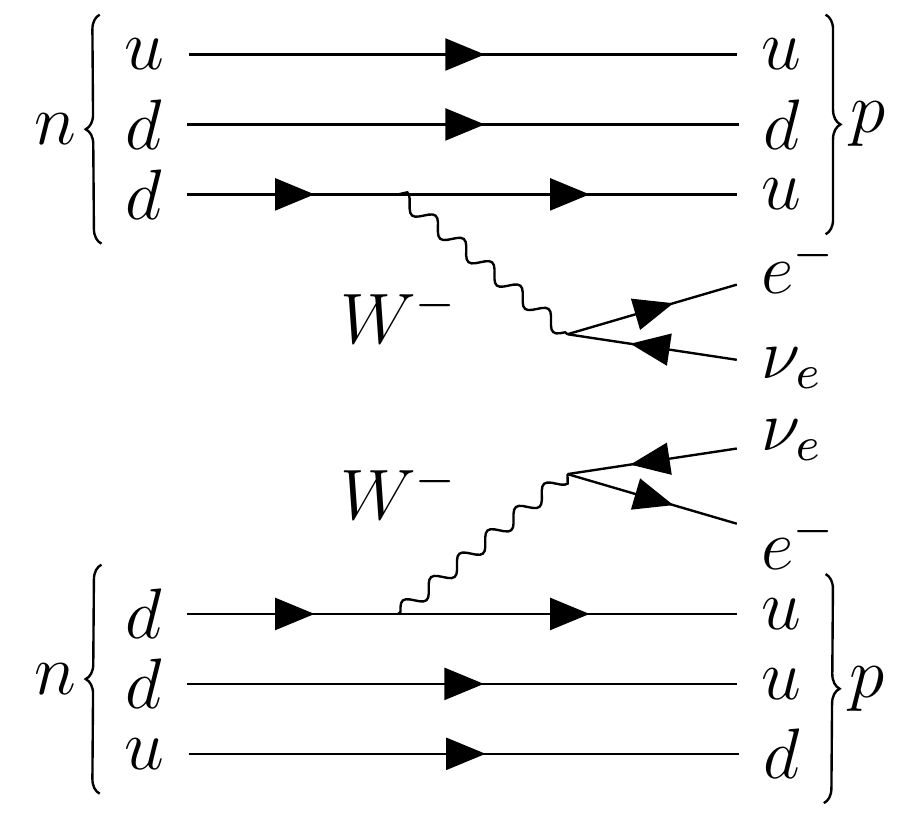
\includegraphics[width=5cm]{doubleBeta2nu_feynman.png}
		\end{minipage}
		\begin{minipage}[t]{0.45\textwidth}{(b)}
			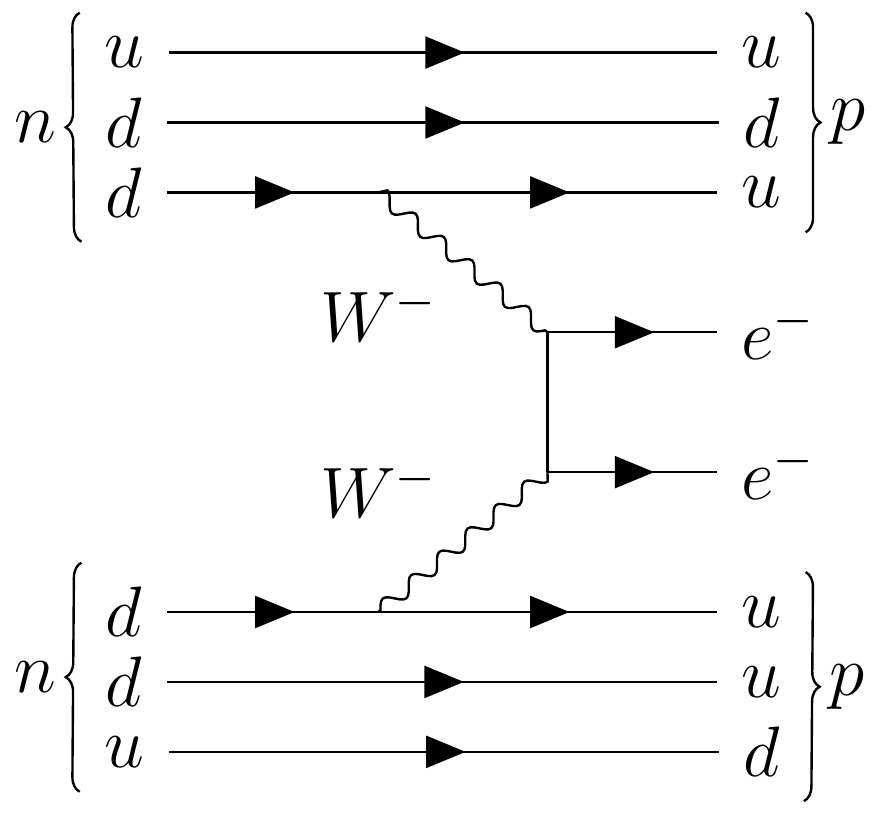
\includegraphics[width=5cm]{doubleBeta_feynman.png}
		\end{minipage}
		\caption{ Feynman diagrams for $2\nu\beta\beta$ (a) and $0\nu\beta\beta$ (b).}
		\label{feynman1}
	}
\end{figure}

Integrating the $\delta t$ with a weight of the nuclear matrix element, the decay width and the half-life are obtained as\cite{suekane2015neutrino,zuber2020neutrino}:
\begin{equation}
\Gamma=(T^{0\nu\beta\beta}_{1/2})^{-1} = G_{PS}(Q,Z)|M_{Nuclear}|^2\langle m_{ee}\rangle^2, 
\end{equation}
where $G_{PS}(Q,Z)$ is a phase space corresponding to the effective coupling constant, which depends on the endpoint energy $Q$ and the atomic number $Z$; $|M_{Nuclear}|$ is the nuclear matrix element describing the nuclear transition and it can only be calculated theoretically from approximate methods based on many-body nuclear models, such as the Nuclear Shell Model (NSM),

